\section{Literature review}
\label{sec:literature review}

Several risk metrics have been developed with the goal of quantifying the risk involved in driving \autocite{minderhoud2001extended, ozbay2008derivation, cunto2009simulated, laureshyn2010evaluation}.
In general, the risk is measured in terms of proximity in time and/or space, ability to perform evasive action like braking or swerving and the magnitude of such actions \autocite{shi2018key,zheng2020modeling}. 
For a collision to occur, the proximity index should be close to zero while the magnitude of evasive actions should be close to the limits of the driver and the vehicle \autocite{zheng2020modeling}. 

Refer to \cref{fig:tux}.

\begin{figure}
    \centering
    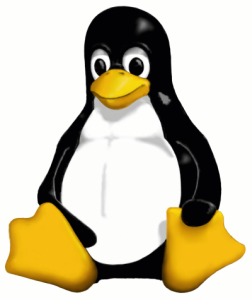
\includegraphics{figs/tux.png}
    \caption{This is an example of a figure.}
    \label{fig:tux}
\end{figure}
